%! Author = wolfram_e_laube
%! Date = 16.04.24

\item[(b)]
The magnitude and phase response of the DTFT is plotted using the following Python code:

\begin{verbatim}
import matplotlib.pyplot as plt
import numpy as np

# Given sequence parameters
n = np.arange(-10, 11)  # Since x[n] is nonzero for n between -10 and 10
x = (0.8)**np.abs(n)

# Frequency vector
w = np.linspace(-np.pi, np.pi, 1000)

# Compute DTFT
X = dtft(x, n, w)

# Plot magnitude and phase response
plt.figure(figsize=(14, 6))

# Magnitude response subplot
plt.subplot(2, 1, 1)
plt.plot(w, np.abs(X))
plt.title('Magnitude Response of $X(e^{j\Omega})$')
plt.xlabel('$\Omega$')
plt.ylabel('|X|')
plt.grid()

# Phase response subplot
plt.subplot(2, 1, 2)
plt.plot(w, np.angle(X))
plt.title('Phase Response of $X(e^{j\Omega})$')
plt.xlabel('$\Omega$')
plt.ylabel('Phase (radians)')
plt.grid()

plt.tight_layout()
plt.show()
\end{verbatim}

This code segment uses Matplotlib to create the plots for the magnitude and phase responses
of the DTFT computed for a discrete sequence.

\begin{figure}[h]
\centering
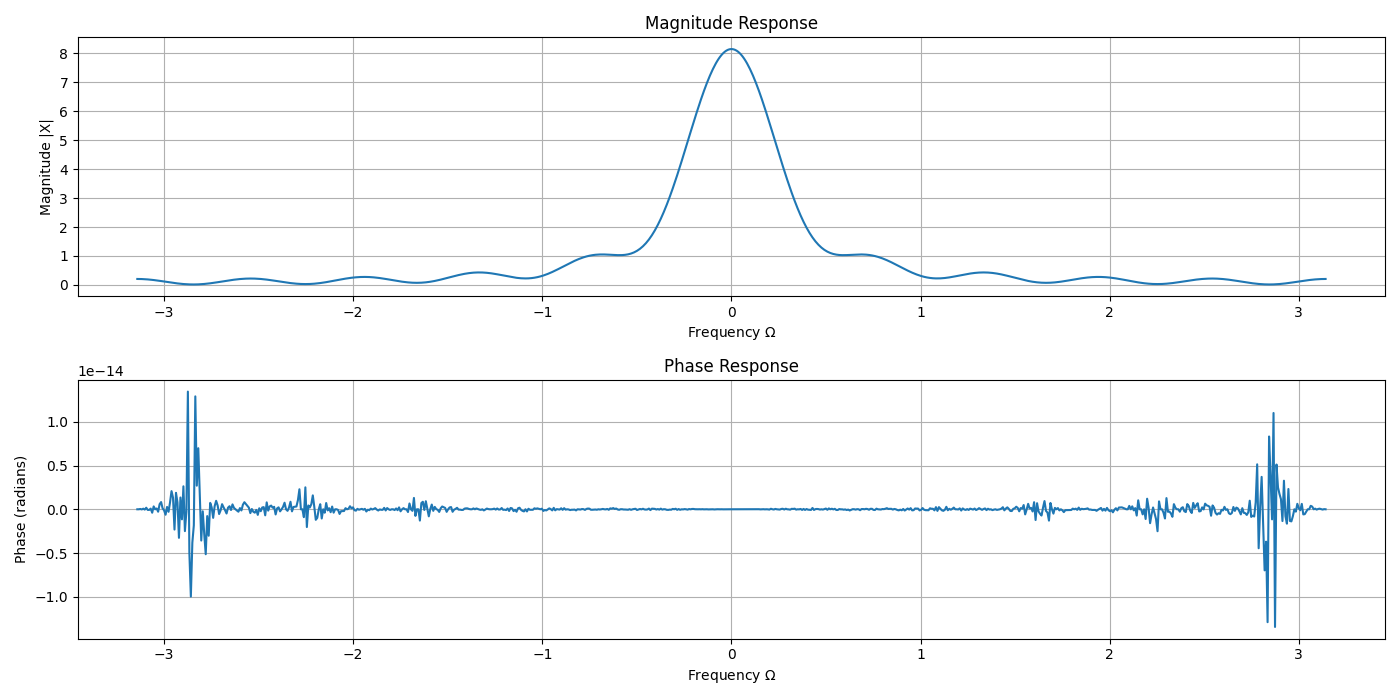
\includegraphics[width=\textwidth]{fig/ex4_b_plot}
\caption{Magnitude and phase of DTFT}
\label{fig:ex4_b_plot}
\end{figure}
